\documentclass[1p]{elsarticle_modified}
%\bibliographystyle{elsarticle-num}

%\usepackage[colorlinks]{hyperref}
%\usepackage{abbrmath_seonhwa} %\Abb, \Ascr, \Acal ,\Abf, \Afrak
\usepackage{amsfonts}
\usepackage{amssymb}
\usepackage{amsmath}
\usepackage{amsthm}
\usepackage{scalefnt}
\usepackage{amsbsy}
\usepackage{kotex}
\usepackage{caption}
\usepackage{subfig}
\usepackage{color}
\usepackage{graphicx}
\usepackage{xcolor} %% white, black, red, green, blue, cyan, magenta, yellow
\usepackage{float}
\usepackage{setspace}
\usepackage{hyperref}

\usepackage{tikz}
\usetikzlibrary{arrows}

\usepackage{multirow}
\usepackage{array} % fixed length table
\usepackage{hhline}

%%%%%%%%%%%%%%%%%%%%%
\makeatletter
\renewcommand*\env@matrix[1][\arraystretch]{%
	\edef\arraystretch{#1}%
	\hskip -\arraycolsep
	\let\@ifnextchar\new@ifnextchar
	\array{*\c@MaxMatrixCols c}}
\makeatother %https://tex.stackexchange.com/questions/14071/how-can-i-increase-the-line-spacing-in-a-matrix
%%%%%%%%%%%%%%%

\usepackage[normalem]{ulem}

\newcommand{\msout}[1]{\ifmmode\text{\sout{\ensuremath{#1}}}\else\sout{#1}\fi}
%SOURCE: \msout is \stkout macro in https://tex.stackexchange.com/questions/20609/strikeout-in-math-mode

\newcommand{\cancel}[1]{
	\ifmmode
	{\color{red}\msout{#1}}
	\else
	{\color{red}\sout{#1}}
	\fi
}

\newcommand{\add}[1]{
	{\color{blue}\uwave{#1}}
}

\newcommand{\replace}[2]{
	\ifmmode
	{\color{red}\msout{#1}}{\color{blue}\uwave{#2}}
	\else
	{\color{red}\sout{#1}}{\color{blue}\uwave{#2}}
	\fi
}

\newcommand{\Sol}{\mathcal{S}} %segment
\newcommand{\D}{D} %diagram
\newcommand{\A}{\mathcal{A}} %arc


%%%%%%%%%%%%%%%%%%%%%%%%%%%%%5 test

\def\sl{\operatorname{\textup{SL}}(2,\Cbb)}
\def\psl{\operatorname{\textup{PSL}}(2,\Cbb)}
\def\quan{\mkern 1mu \triangleright \mkern 1mu}

\theoremstyle{definition}
\newtheorem{thm}{Theorem}[section]
\newtheorem{prop}[thm]{Proposition}
\newtheorem{lem}[thm]{Lemma}
\newtheorem{ques}[thm]{Question}
\newtheorem{cor}[thm]{Corollary}
\newtheorem{defn}[thm]{Definition}
\newtheorem{exam}[thm]{Example}
\newtheorem{rmk}[thm]{Remark}
\newtheorem{alg}[thm]{Algorithm}

\newcommand{\I}{\sqrt{-1}}
\begin{document}

%\begin{frontmatter}
%
%\title{Boundary parabolic representations of knots up to 8 crossings}
%
%%% Group authors per affiliation:
%\author{Yunhi Cho} 
%\address{Department of Mathematics, University of Seoul, Seoul, Korea}
%\ead{yhcho@uos.ac.kr}
%
%
%\author{Seonhwa Kim} %\fnref{s_kim}}
%\address{Center for Geometry and Physics, Institute for Basic Science, Pohang, 37673, Korea}
%\ead{ryeona17@ibs.re.kr}
%
%\author{Hyuk Kim}
%\address{Department of Mathematical Sciences, Seoul National University, Seoul 08826, Korea}
%\ead{hyukkim@snu.ac.kr}
%
%\author{Seokbeom Yoon}
%\address{Department of Mathematical Sciences, Seoul National University, Seoul, 08826,  Korea}
%\ead{sbyoon15@snu.ac.kr}
%
%\begin{abstract}
%We find all boundary parabolic representation of knots up to 8 crossings.
%
%\end{abstract}
%\begin{keyword}
%    \MSC[2010] 57M25 
%\end{keyword}
%
%\end{frontmatter}

%\linenumbers
%\tableofcontents
%
\newcommand\colored[1]{\textcolor{white}{\rule[-0.35ex]{0.8em}{1.4ex}}\kern-0.8em\color{red} #1}%
%\newcommand\colored[1]{\textcolor{white}{ #1}\kern-2.17ex	\textcolor{white}{ #1}\kern-1.81ex	\textcolor{white}{ #1}\kern-2.15ex\color{red}#1	}

{\Large $\underline{12n_{0116}~(K12n_{0116})}$}

\setlength{\tabcolsep}{10pt}
\renewcommand{\arraystretch}{1.6}
\vspace{1cm}\begin{tabular}{m{100pt}>{\centering\arraybackslash}m{274pt}}
\multirow{5}{120pt}{
	\centering
	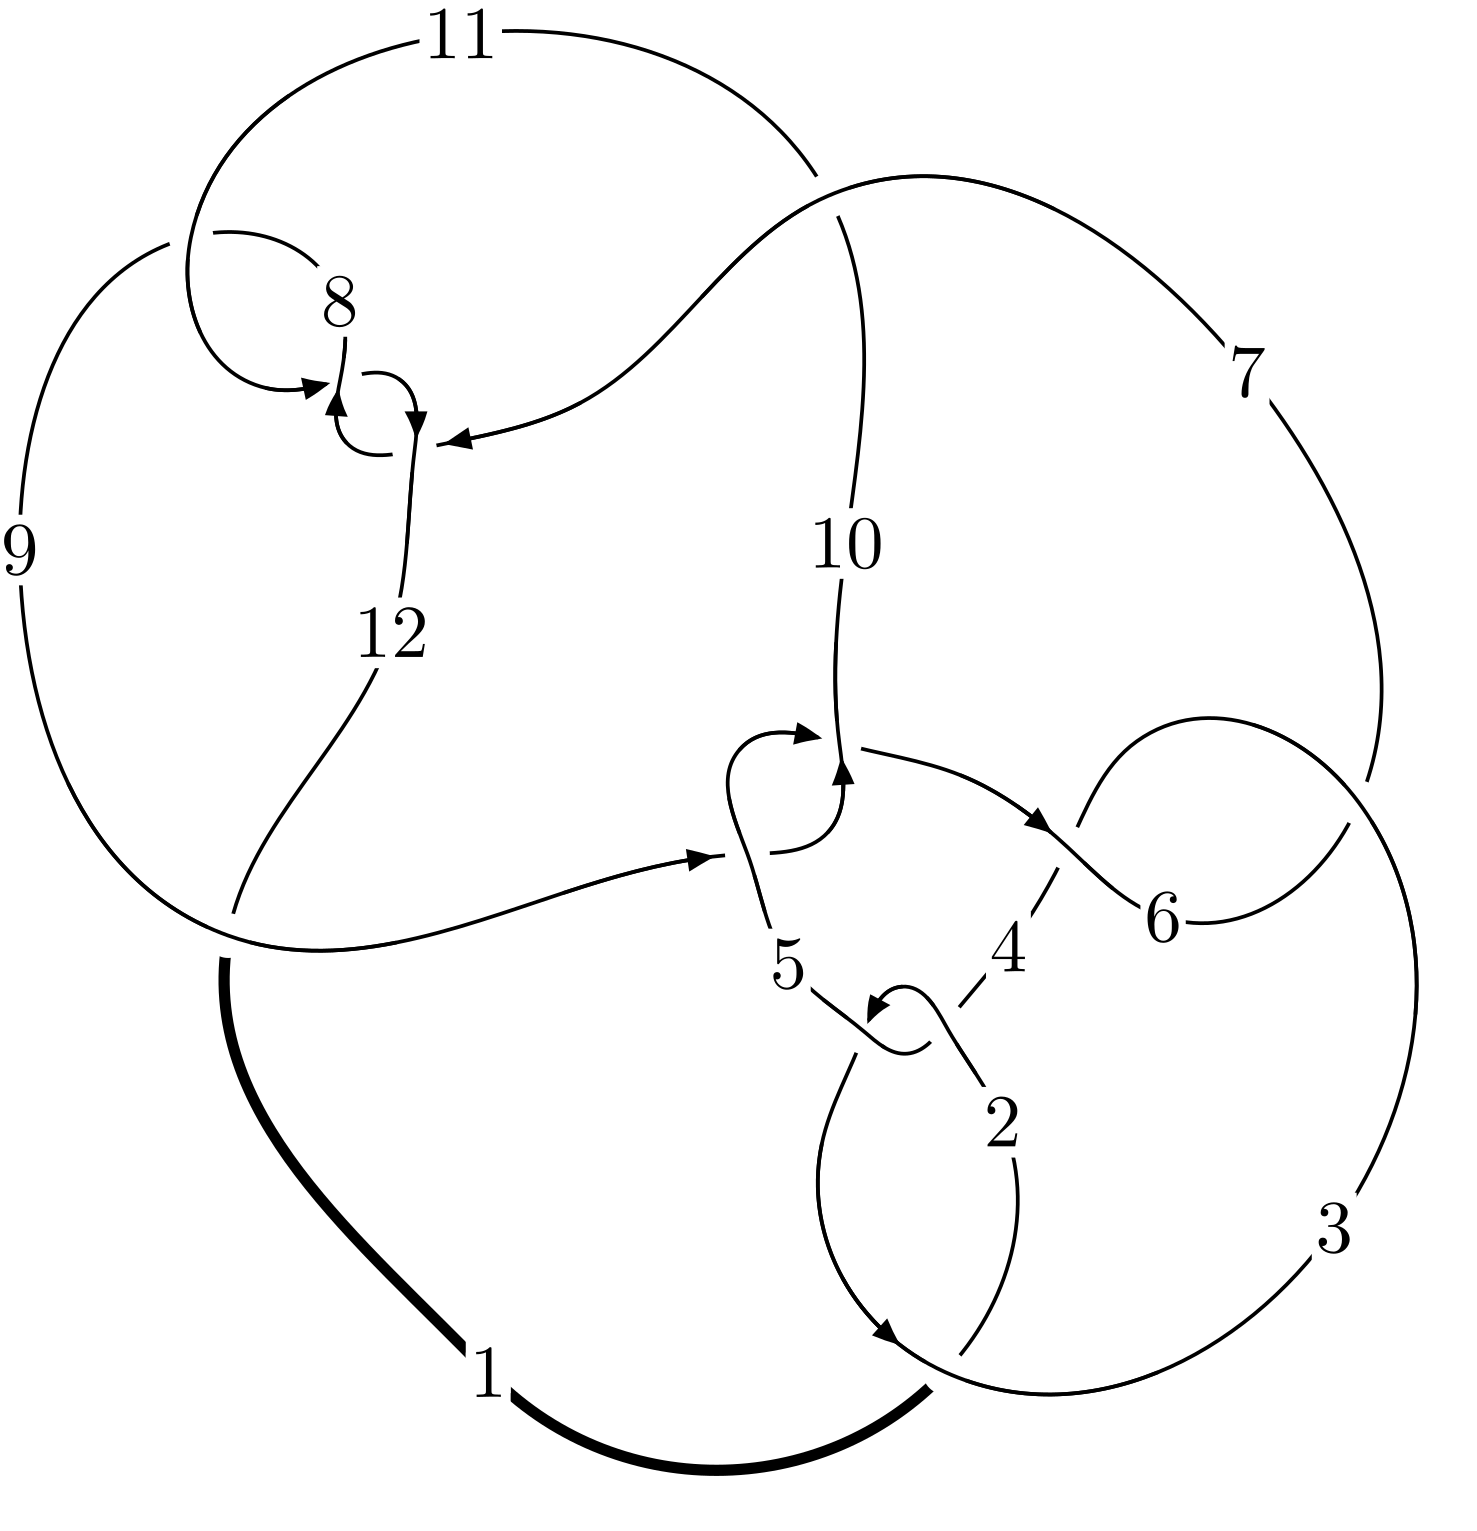
\includegraphics[width=112pt]{../../../GIT/diagram.site/Diagrams/png/2205_12n_0116.png}\\
\ \ \ A knot diagram\footnotemark}&
\allowdisplaybreaks
\textbf{Linearized knot diagam} \\
\cline{2-2}
 &
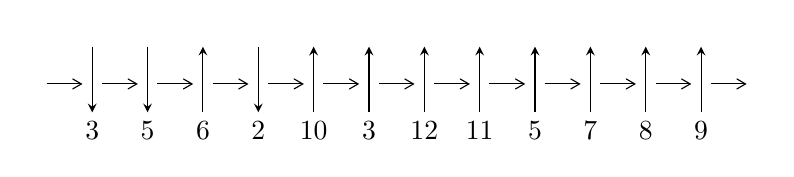
\begin{tikzpicture}[x=20pt, y=17pt]
	% nodes
	\node (C0) at (0, 0) {};
	\node (C1) at (1, 0) {};
	\node (C1U) at (1, +1) {};
	\node (C1D) at (1, -1) {3};

	\node (C2) at (2, 0) {};
	\node (C2U) at (2, +1) {};
	\node (C2D) at (2, -1) {5};

	\node (C3) at (3, 0) {};
	\node (C3U) at (3, +1) {};
	\node (C3D) at (3, -1) {6};

	\node (C4) at (4, 0) {};
	\node (C4U) at (4, +1) {};
	\node (C4D) at (4, -1) {2};

	\node (C5) at (5, 0) {};
	\node (C5U) at (5, +1) {};
	\node (C5D) at (5, -1) {10};

	\node (C6) at (6, 0) {};
	\node (C6U) at (6, +1) {};
	\node (C6D) at (6, -1) {3};

	\node (C7) at (7, 0) {};
	\node (C7U) at (7, +1) {};
	\node (C7D) at (7, -1) {12};

	\node (C8) at (8, 0) {};
	\node (C8U) at (8, +1) {};
	\node (C8D) at (8, -1) {11};

	\node (C9) at (9, 0) {};
	\node (C9U) at (9, +1) {};
	\node (C9D) at (9, -1) {5};

	\node (C10) at (10, 0) {};
	\node (C10U) at (10, +1) {};
	\node (C10D) at (10, -1) {7};

	\node (C11) at (11, 0) {};
	\node (C11U) at (11, +1) {};
	\node (C11D) at (11, -1) {8};

	\node (C12) at (12, 0) {};
	\node (C12U) at (12, +1) {};
	\node (C12D) at (12, -1) {9};
	\node (C13) at (13, 0) {};

	% arrows
	\draw[->,>={angle 60}]
	(C0) edge (C1) (C1) edge (C2) (C2) edge (C3) (C3) edge (C4) (C4) edge (C5) (C5) edge (C6) (C6) edge (C7) (C7) edge (C8) (C8) edge (C9) (C9) edge (C10) (C10) edge (C11) (C11) edge (C12) (C12) edge (C13) ;	\draw[->,>=stealth]
	(C1U) edge (C1D) (C2U) edge (C2D) (C3D) edge (C3U) (C4U) edge (C4D) (C5D) edge (C5U) (C6D) edge (C6U) (C7D) edge (C7U) (C8D) edge (C8U) (C9D) edge (C9U) (C10D) edge (C10U) (C11D) edge (C11U) (C12D) edge (C12U) ;
	\end{tikzpicture} \\
\hhline{~~} \\& 
\textbf{Solving Sequence} \\ \cline{2-2} 
 &
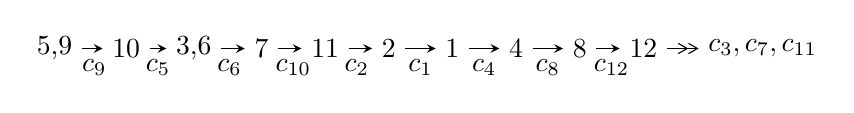
\begin{tikzpicture}[x=23pt, y=7pt]
	% node
	\node (A0) at (-1/8, 0) {5,9};
	\node (A1) at (1, 0) {10};
	\node (A2) at (33/16, 0) {3,6};
	\node (A3) at (25/8, 0) {7};
	\node (A4) at (33/8, 0) {11};
	\node (A5) at (41/8, 0) {2};
	\node (A6) at (49/8, 0) {1};
	\node (A7) at (57/8, 0) {4};
	\node (A8) at (65/8, 0) {8};
	\node (A9) at (73/8, 0) {12};
	\node (C1) at (1/2, -1) {$c_{9}$};
	\node (C2) at (3/2, -1) {$c_{5}$};
	\node (C3) at (21/8, -1) {$c_{6}$};
	\node (C4) at (29/8, -1) {$c_{10}$};
	\node (C5) at (37/8, -1) {$c_{2}$};
	\node (C6) at (45/8, -1) {$c_{1}$};
	\node (C7) at (53/8, -1) {$c_{4}$};
	\node (C8) at (61/8, -1) {$c_{8}$};
	\node (C9) at (69/8, -1) {$c_{12}$};
	\node (A10) at (11, 0) {$c_{3},c_{7},c_{11}$};

	% edge
	\draw[->,>=stealth]	
	(A0) edge (A1) (A1) edge (A2) (A2) edge (A3) (A3) edge (A4) (A4) edge (A5) (A5) edge (A6) (A6) edge (A7) (A7) edge (A8) (A8) edge (A9) ;
	\draw[->>,>={angle 60}]	
	(A9) edge (A10);
\end{tikzpicture} \\ 

\end{tabular} \\

\footnotetext{
The image of knot diagram is generated by the software ``\textbf{Draw programme}" developed by Andrew Bartholomew(\url{http://www.layer8.co.uk/maths/draw/index.htm\#Running-draw}), where we modified some parts for our purpose(\url{https://github.com/CATsTAILs/LinksPainter}).
}\phantom \\ \newline 
\centering \textbf{Ideals for irreducible components\footnotemark of $X_{\text{par}}$} 
 
\begin{align*}
I^u_{1}&=\langle 
-1.49041\times10^{48} u^{40}-1.63923\times10^{48} u^{39}+\cdots+4.94994\times10^{48} b+1.35928\times10^{48},\\
\phantom{I^u_{1}}&\phantom{= \langle  }-1.49041\times10^{48} u^{40}-1.63923\times10^{48} u^{39}+\cdots+4.94994\times10^{48} a+1.35928\times10^{48},\;u^{41}+2 u^{40}+\cdots- u-1\rangle \\
I^u_{2}&=\langle 
- u^5+u^4+3 u^3-2 u^2+b- u-1,\;- u^5+u^4+3 u^3-2 u^2+a-2 u-1,\;u^6- u^5-3 u^4+2 u^3+2 u^2+u-1\rangle \\
\\
\end{align*}
\raggedright * 2 irreducible components of $\dim_{\mathbb{C}}=0$, with total 47 representations.\\
\footnotetext{All coefficients of polynomials are rational numbers. But the coefficients are sometimes approximated in decimal forms when there is not enough margin.}
\newpage
\renewcommand{\arraystretch}{1}
\centering \section*{I. $I^u_{1}= \langle -1.49\times10^{48} u^{40}-1.64\times10^{48} u^{39}+\cdots+4.95\times10^{48} b+1.36\times10^{48},\;-1.49\times10^{48} u^{40}-1.64\times10^{48} u^{39}+\cdots+4.95\times10^{48} a+1.36\times10^{48},\;u^{41}+2 u^{40}+\cdots- u-1 \rangle$}
\flushleft \textbf{(i) Arc colorings}\\
\begin{tabular}{m{7pt} m{180pt} m{7pt} m{180pt} }
\flushright $a_{5}=$&$\begin{pmatrix}0\\u\end{pmatrix}$ \\
\flushright $a_{9}=$&$\begin{pmatrix}1\\0\end{pmatrix}$ \\
\flushright $a_{10}=$&$\begin{pmatrix}1\\- u^2\end{pmatrix}$ \\
\flushright $a_{3}=$&$\begin{pmatrix}0.301096 u^{40}+0.331162 u^{39}+\cdots+2.34511 u-0.274605\\0.301096 u^{40}+0.331162 u^{39}+\cdots+3.34511 u-0.274605\end{pmatrix}$ \\
\flushright $a_{6}=$&$\begin{pmatrix}u\\- u^3+u\end{pmatrix}$ \\
\flushright $a_{7}=$&$\begin{pmatrix}-0.501619 u^{40}-0.639447 u^{39}+\cdots+0.896473 u+0.455440\\-0.458393 u^{40}-0.639616 u^{39}+\cdots+0.799469 u+0.637044\end{pmatrix}$ \\
\flushright $a_{11}=$&$\begin{pmatrix}-0.205384 u^{40}-0.351951 u^{39}+\cdots+0.606975 u+1.47006\\-0.559530 u^{40}-0.970963 u^{39}+\cdots+1.39792 u+1.11199\end{pmatrix}$ \\
\flushright $a_{2}=$&$\begin{pmatrix}0.301096 u^{40}+0.331162 u^{39}+\cdots+2.34511 u-0.274605\\0.0224886 u^{40}-0.0444496 u^{39}+\cdots+3.31504 u-0.00357471\end{pmatrix}$ \\
\flushright $a_{1}=$&$\begin{pmatrix}0.110835 u^{40}-0.0229094 u^{39}+\cdots-0.234831 u+0.545396\\-0.390784 u^{40}-0.662356 u^{39}+\cdots+0.661642 u+1.00084\end{pmatrix}$ \\
\flushright $a_{4}=$&$\begin{pmatrix}0.257870 u^{40}+0.331331 u^{39}+\cdots+2.44211 u-0.456209\\0.313467 u^{40}+0.443108 u^{39}+\cdots+3.39872 u-0.542830\end{pmatrix}$ \\
\flushright $a_{8}=$&$\begin{pmatrix}-0.659770 u^{40}-1.09530 u^{39}+\cdots+1.32120 u+1.69134\\-0.119568 u^{40}+0.0303721 u^{39}+\cdots-0.186514 u-1.02623\end{pmatrix}$ \\
\flushright $a_{12}=$&$\begin{pmatrix}0.501619 u^{40}+0.639447 u^{39}+\cdots-0.896473 u-0.455440\\-0.390784 u^{40}-0.662356 u^{39}+\cdots+0.661642 u+1.00084\end{pmatrix}$\\&\end{tabular}
\flushleft \textbf{(ii) Obstruction class $= -1$}\\~\\
\flushleft \textbf{(iii) Cusp Shapes $= -4.91398 u^{40}-6.25021 u^{39}+\cdots-14.4903 u+31.2535$}\\~\\
\newpage\renewcommand{\arraystretch}{1}
\flushleft \textbf{(iv) u-Polynomials at the component}\newline \\
\begin{tabular}{m{50pt}|m{274pt}}
Crossings & \hspace{64pt}u-Polynomials at each crossing \\
\hline $$\begin{aligned}c_{1}\end{aligned}$$&$\begin{aligned}
&u^{41}+47 u^{40}+\cdots+296 u+1
\end{aligned}$\\
\hline $$\begin{aligned}c_{2},c_{4}\end{aligned}$$&$\begin{aligned}
&u^{41}-7 u^{40}+\cdots-12 u+1
\end{aligned}$\\
\hline $$\begin{aligned}c_{3},c_{6}\end{aligned}$$&$\begin{aligned}
&u^{41}+7 u^{40}+\cdots+640 u-64
\end{aligned}$\\
\hline $$\begin{aligned}c_{5},c_{9}\end{aligned}$$&$\begin{aligned}
&u^{41}+2 u^{40}+\cdots- u-1
\end{aligned}$\\
\hline $$\begin{aligned}c_{7},c_{8},c_{11}\end{aligned}$$&$\begin{aligned}
&u^{41}+2 u^{40}+\cdots+u+1
\end{aligned}$\\
\hline $$\begin{aligned}c_{10},c_{12}\end{aligned}$$&$\begin{aligned}
&u^{41}-2 u^{40}+\cdots-47 u+17
\end{aligned}$\\
\hline
\end{tabular}\\~\\
\newpage\renewcommand{\arraystretch}{1}
\flushleft \textbf{(v) Riley Polynomials at the component}\newline \\
\begin{tabular}{m{50pt}|m{274pt}}
Crossings & \hspace{64pt}Riley Polynomials at each crossing \\
\hline $$\begin{aligned}c_{1}\end{aligned}$$&$\begin{aligned}
&y^{41}-99 y^{40}+\cdots+111528 y-1
\end{aligned}$\\
\hline $$\begin{aligned}c_{2},c_{4}\end{aligned}$$&$\begin{aligned}
&y^{41}-47 y^{40}+\cdots+296 y-1
\end{aligned}$\\
\hline $$\begin{aligned}c_{3},c_{6}\end{aligned}$$&$\begin{aligned}
&y^{41}+39 y^{40}+\cdots+90112 y-4096
\end{aligned}$\\
\hline $$\begin{aligned}c_{5},c_{9}\end{aligned}$$&$\begin{aligned}
&y^{41}+42 y^{39}+\cdots+7 y-1
\end{aligned}$\\
\hline $$\begin{aligned}c_{7},c_{8},c_{11}\end{aligned}$$&$\begin{aligned}
&y^{41}+36 y^{40}+\cdots+7 y-1
\end{aligned}$\\
\hline $$\begin{aligned}c_{10},c_{12}\end{aligned}$$&$\begin{aligned}
&y^{41}-12 y^{40}+\cdots-2041 y-289
\end{aligned}$\\
\hline
\end{tabular}\\~\\
\newpage\flushleft \textbf{(vi) Complex Volumes and Cusp Shapes}
$$\begin{array}{c|c|c}  
\text{Solutions to }I^u_{1}& \I (\text{vol} + \sqrt{-1}CS) & \text{Cusp shape}\\
 \hline 
\begin{aligned}
u &= -0.546127 + 0.811291 I \\
a &= \phantom{-}0.743645 - 1.202480 I \\
b &= \phantom{-}0.197518 - 0.391191 I\end{aligned}
 & -4.83591 - 7.62929 I & \phantom{-}1.63110 + 8.21040 I \\ \hline\begin{aligned}
u &= -0.546127 - 0.811291 I \\
a &= \phantom{-}0.743645 + 1.202480 I \\
b &= \phantom{-}0.197518 + 0.391191 I\end{aligned}
 & -4.83591 + 7.62929 I & \phantom{-}1.63110 - 8.21040 I \\ \hline\begin{aligned}
u &= \phantom{-}0.559771 + 0.753240 I \\
a &= -0.624352 - 1.085930 I \\
b &= -0.064581 - 0.332685 I\end{aligned}
 & \phantom{-}0.18158 + 4.25829 I & \phantom{-}7.22708 - 8.04646 I \\ \hline\begin{aligned}
u &= \phantom{-}0.559771 - 0.753240 I \\
a &= -0.624352 + 1.085930 I \\
b &= -0.064581 + 0.332685 I\end{aligned}
 & \phantom{-}0.18158 - 4.25829 I & \phantom{-}7.22708 + 8.04646 I \\ \hline\begin{aligned}
u &= -0.664122 + 0.603424 I \\
a &= \phantom{-}0.468587 - 0.663053 I \\
b &= -0.195535 - 0.059628 I\end{aligned}
 & -2.14123 - 1.43316 I & \phantom{-}6.02200 + 3.64151 I \\ \hline\begin{aligned}
u &= -0.664122 - 0.603424 I \\
a &= \phantom{-}0.468587 + 0.663053 I \\
b &= -0.195535 + 0.059628 I\end{aligned}
 & -2.14123 + 1.43316 I & \phantom{-}6.02200 - 3.64151 I \\ \hline\begin{aligned}
u &= \phantom{-}0.350975 + 0.790999 I \\
a &= -0.39756 - 1.62860 I \\
b &= -0.046582 - 0.837603 I\end{aligned}
 & -6.73300 + 0.22938 I & -2.25086 - 2.33731 I \\ \hline\begin{aligned}
u &= \phantom{-}0.350975 - 0.790999 I \\
a &= -0.39756 + 1.62860 I \\
b &= -0.046582 + 0.837603 I\end{aligned}
 & -6.73300 - 0.22938 I & -2.25086 + 2.33731 I \\ \hline\begin{aligned}
u &= \phantom{-}0.087719 + 0.850756 I \\
a &= -0.12108 - 2.10269 I \\
b &= -0.033358 - 1.251940 I\end{aligned}
 & -8.03114 + 3.86698 I & -3.56668 - 3.96784 I \\ \hline\begin{aligned}
u &= \phantom{-}0.087719 - 0.850756 I \\
a &= -0.12108 + 2.10269 I \\
b &= -0.033358 + 1.251940 I\end{aligned}
 & -8.03114 - 3.86698 I & -3.56668 + 3.96784 I\\
 \hline 
 \end{array}$$\newpage$$\begin{array}{c|c|c}  
\text{Solutions to }I^u_{1}& \I (\text{vol} + \sqrt{-1}CS) & \text{Cusp shape}\\
 \hline 
\begin{aligned}
u &= -0.445566 + 0.616611 I \\
a &= \phantom{-}0.112439 - 1.137990 I \\
b &= -0.333128 - 0.521377 I\end{aligned}
 & -1.53709 - 1.40851 I & \phantom{-}1.34634 + 3.01002 I \\ \hline\begin{aligned}
u &= -0.445566 - 0.616611 I \\
a &= \phantom{-}0.112439 + 1.137990 I \\
b &= -0.333128 + 0.521377 I\end{aligned}
 & -1.53709 + 1.40851 I & \phantom{-}1.34634 - 3.01002 I \\ \hline\begin{aligned}
u &= -0.090722 + 0.752674 I \\
a &= \phantom{-}0.05605 - 1.99845 I \\
b &= -0.034673 - 1.245770 I\end{aligned}
 & -2.86548 - 1.28813 I & \phantom{-}1.16839 + 4.84793 I \\ \hline\begin{aligned}
u &= -0.090722 - 0.752674 I \\
a &= \phantom{-}0.05605 + 1.99845 I \\
b &= -0.034673 + 1.245770 I\end{aligned}
 & -2.86548 + 1.28813 I & \phantom{-}1.16839 - 4.84793 I \\ \hline\begin{aligned}
u &= -0.527293 + 0.436682 I \\
a &= -0.973519 - 0.176954 I \\
b &= -1.50081 + 0.25973 I\end{aligned}
 & -4.01492 + 3.79256 I & \phantom{-}2.77393 - 0.06472 I \\ \hline\begin{aligned}
u &= -0.527293 - 0.436682 I \\
a &= -0.973519 + 0.176954 I \\
b &= -1.50081 - 0.25973 I\end{aligned}
 & -4.01492 - 3.79256 I & \phantom{-}2.77393 + 0.06472 I \\ \hline\begin{aligned}
u &= \phantom{-}0.468495 + 0.464998 I \\
a &= \phantom{-}0.622134 - 0.271062 I \\
b &= \phantom{-}1.090630 + 0.193936 I\end{aligned}
 & \phantom{-}0.599224 - 0.610593 I & \phantom{-}8.50615 - 0.01136 I \\ \hline\begin{aligned}
u &= \phantom{-}0.468495 - 0.464998 I \\
a &= \phantom{-}0.622134 + 0.271062 I \\
b &= \phantom{-}1.090630 - 0.193936 I\end{aligned}
 & \phantom{-}0.599224 + 0.610593 I & \phantom{-}8.50615 + 0.01136 I \\ \hline\begin{aligned}
u &= -0.325958 + 0.548034 I \\
a &= -0.267538 + 0.084708 I \\
b &= -0.593496 + 0.632743 I\end{aligned}
 & -2.79420 - 2.18222 I & \phantom{-}4.51636 + 3.99594 I \\ \hline\begin{aligned}
u &= -0.325958 - 0.548034 I \\
a &= -0.267538 - 0.084708 I \\
b &= -0.593496 - 0.632743 I\end{aligned}
 & -2.79420 + 2.18222 I & \phantom{-}4.51636 - 3.99594 I\\
 \hline 
 \end{array}$$\newpage$$\begin{array}{c|c|c}  
\text{Solutions to }I^u_{1}& \I (\text{vol} + \sqrt{-1}CS) & \text{Cusp shape}\\
 \hline 
\begin{aligned}
u &= \phantom{-}1.397250 + 0.182037 I \\
a &= -0.506275 - 0.004273 I \\
b &= \phantom{-}0.890974 + 0.177764 I\end{aligned}
 & \phantom{-}2.57061 + 4.43167 I & \phantom{-}14.03660 + 0. I\phantom{ +0.000000I} \\ \hline\begin{aligned}
u &= \phantom{-}1.397250 - 0.182037 I \\
a &= -0.506275 + 0.004273 I \\
b &= \phantom{-}0.890974 - 0.177764 I\end{aligned}
 & \phantom{-}2.57061 - 4.43167 I & \phantom{-}14.03660 + 0. I\phantom{ +0.000000I} \\ \hline\begin{aligned}
u &= -1.41231\phantom{ +0.000000I} \\
a &= \phantom{-}0.496036\phantom{ +0.000000I} \\
b &= -0.916272\phantom{ +0.000000I}\end{aligned}
 & \phantom{-}6.54065\phantom{ +0.000000I} & \phantom{-}18.5250\phantom{ +0.000000I} \\ \hline\begin{aligned}
u &= \phantom{-}0.487776 + 0.155470 I \\
a &= \phantom{-}2.02925 - 0.39422 I \\
b &= \phantom{-}2.51703 - 0.23875 I\end{aligned}
 & -4.99926 + 2.47497 I & \phantom{-}10.9995 - 16.9397 I \\ \hline\begin{aligned}
u &= \phantom{-}0.487776 - 0.155470 I \\
a &= \phantom{-}2.02925 + 0.39422 I \\
b &= \phantom{-}2.51703 + 0.23875 I\end{aligned}
 & -4.99926 - 2.47497 I & \phantom{-}10.9995 + 16.9397 I \\ \hline\begin{aligned}
u &= \phantom{-}0.497461\phantom{ +0.000000I} \\
a &= -0.110298\phantom{ +0.000000I} \\
b &= \phantom{-}0.387162\phantom{ +0.000000I}\end{aligned}
 & \phantom{-}0.683544\phantom{ +0.000000I} & \phantom{-}14.8150\phantom{ +0.000000I} \\ \hline\begin{aligned}
u &= -1.05090 + 1.14678 I \\
a &= \phantom{-}0.504687 + 0.968425 I \\
b &= -0.54621 + 2.11520 I\end{aligned}
 & -11.9065 - 13.7324 I & \phantom{-0.000000 } 0 \\ \hline\begin{aligned}
u &= -1.05090 - 1.14678 I \\
a &= \phantom{-}0.504687 - 0.968425 I \\
b &= -0.54621 - 2.11520 I\end{aligned}
 & -11.9065 + 13.7324 I & \phantom{-0.000000 } 0 \\ \hline\begin{aligned}
u &= \phantom{-}1.05595 + 1.16152 I \\
a &= -0.501764 + 0.917028 I \\
b &= \phantom{-}0.55418 + 2.07855 I\end{aligned}
 & -6.55369 + 9.57234 I & \phantom{-0.000000 } 0 \\ \hline\begin{aligned}
u &= \phantom{-}1.05595 - 1.16152 I \\
a &= -0.501764 - 0.917028 I \\
b &= \phantom{-}0.55418 - 2.07855 I\end{aligned}
 & -6.55369 - 9.57234 I & \phantom{-0.000000 } 0\\
 \hline 
 \end{array}$$\newpage$$\begin{array}{c|c|c}  
\text{Solutions to }I^u_{1}& \I (\text{vol} + \sqrt{-1}CS) & \text{Cusp shape}\\
 \hline 
\begin{aligned}
u &= \phantom{-}1.10127 + 1.14227 I \\
a &= -0.673483 + 0.861835 I \\
b &= \phantom{-}0.42779 + 2.00411 I\end{aligned}
 & -16.5464 + 4.1585 I & \phantom{-0.000000 } 0 \\ \hline\begin{aligned}
u &= \phantom{-}1.10127 - 1.14227 I \\
a &= -0.673483 - 0.861835 I \\
b &= \phantom{-}0.42779 - 2.00411 I\end{aligned}
 & -16.5464 - 4.1585 I & \phantom{-0.000000 } 0 \\ \hline\begin{aligned}
u &= -1.07763 + 1.17451 I \\
a &= \phantom{-}0.535143 + 0.849624 I \\
b &= -0.54248 + 2.02413 I\end{aligned}
 & -8.52808 - 4.96231 I & \phantom{-0.000000 } 0 \\ \hline\begin{aligned}
u &= -1.07763 - 1.17451 I \\
a &= \phantom{-}0.535143 - 0.849624 I \\
b &= -0.54248 - 2.02413 I\end{aligned}
 & -8.52808 + 4.96231 I & \phantom{-0.000000 } 0 \\ \hline\begin{aligned}
u &= -1.16301 + 1.12527 I \\
a &= \phantom{-}0.754065 + 0.641582 I \\
b &= -0.40895 + 1.76685 I\end{aligned}
 & -11.60780 + 5.44383 I & \phantom{-0.000000 } 0 \\ \hline\begin{aligned}
u &= -1.16301 - 1.12527 I \\
a &= \phantom{-}0.754065 - 0.641582 I \\
b &= -0.40895 - 1.76685 I\end{aligned}
 & -11.60780 - 5.44383 I & \phantom{-0.000000 } 0 \\ \hline\begin{aligned}
u &= -0.373875\phantom{ +0.000000I} \\
a &= -2.77728\phantom{ +0.000000I} \\
b &= -3.15116\phantom{ +0.000000I}\end{aligned}
 & -0.771990\phantom{ +0.000000I} & \phantom{-}64.9410\phantom{ +0.000000I} \\ \hline\begin{aligned}
u &= -1.13639 + 1.17348 I \\
a &= \phantom{-}0.623222 + 0.717077 I \\
b &= -0.51317 + 1.89056 I\end{aligned}
 & -8.37413 - 3.52292 I & \phantom{-0.000000 } 0 \\ \hline\begin{aligned}
u &= -1.13639 - 1.17348 I \\
a &= \phantom{-}0.623222 - 0.717077 I \\
b &= -0.51317 - 1.89056 I\end{aligned}
 & -8.37413 + 3.52292 I & \phantom{-0.000000 } 0 \\ \hline\begin{aligned}
u &= \phantom{-}1.16288 + 1.15013 I \\
a &= -0.687885 + 0.655673 I \\
b &= \phantom{-}0.47499 + 1.80580 I\end{aligned}
 & -6.27214 - 1.18033 I & \phantom{-0.000000 } 0\\
 \hline 
 \end{array}$$\newpage$$\begin{array}{c|c|c}  
\text{Solutions to }I^u_{1}& \I (\text{vol} + \sqrt{-1}CS) & \text{Cusp shape}\\
 \hline 
\begin{aligned}
u &= \phantom{-}1.16288 - 1.15013 I \\
a &= -0.687885 - 0.655673 I \\
b &= \phantom{-}0.47499 - 1.80580 I\end{aligned}
 & -6.27214 + 1.18033 I & \phantom{-0.000000 } 0\\
 \hline 
 \end{array}$$\newpage\newpage\renewcommand{\arraystretch}{1}
\centering \section*{II. $I^u_{2}= \langle - u^5+u^4+3 u^3-2 u^2+b- u-1,\;- u^5+u^4+3 u^3-2 u^2+a-2 u-1,\;u^6- u^5-3 u^4+2 u^3+2 u^2+u-1 \rangle$}
\flushleft \textbf{(i) Arc colorings}\\
\begin{tabular}{m{7pt} m{180pt} m{7pt} m{180pt} }
\flushright $a_{5}=$&$\begin{pmatrix}0\\u\end{pmatrix}$ \\
\flushright $a_{9}=$&$\begin{pmatrix}1\\0\end{pmatrix}$ \\
\flushright $a_{10}=$&$\begin{pmatrix}1\\- u^2\end{pmatrix}$ \\
\flushright $a_{3}=$&$\begin{pmatrix}u^5- u^4-3 u^3+2 u^2+2 u+1\\u^5- u^4-3 u^3+2 u^2+u+1\end{pmatrix}$ \\
\flushright $a_{6}=$&$\begin{pmatrix}u\\- u^3+u\end{pmatrix}$ \\
\flushright $a_{7}=$&$\begin{pmatrix}u\\- u^3+u\end{pmatrix}$ \\
\flushright $a_{11}=$&$\begin{pmatrix}- u^2+1\\u^4-2 u^2\end{pmatrix}$ \\
\flushright $a_{2}=$&$\begin{pmatrix}u^5- u^4-3 u^3+2 u^2+2 u+1\\u^5- u^4-3 u^3+2 u^2+1\end{pmatrix}$ \\
\flushright $a_{1}=$&$\begin{pmatrix}0\\- u\end{pmatrix}$ \\
\flushright $a_{4}=$&$\begin{pmatrix}u^5- u^4-3 u^3+2 u^2+2 u+1\\u^5- u^4-3 u^3+2 u^2+u+1\end{pmatrix}$ \\
\flushright $a_{8}=$&$\begin{pmatrix}- u^5+2 u^3+u\\u^5-3 u^3+u\end{pmatrix}$ \\
\flushright $a_{12}=$&$\begin{pmatrix}u\\- u\end{pmatrix}$\\&\end{tabular}
\flushleft \textbf{(ii) Obstruction class $= 1$}\\~\\
\flushleft \textbf{(iii) Cusp Shapes $= -7 u^5+3 u^4+19 u^3-5 u^2-8 u-6$}\\~\\
\newpage\renewcommand{\arraystretch}{1}
\flushleft \textbf{(iv) u-Polynomials at the component}\newline \\
\begin{tabular}{m{50pt}|m{274pt}}
Crossings & \hspace{64pt}u-Polynomials at each crossing \\
\hline $$\begin{aligned}c_{1},c_{2}\end{aligned}$$&$\begin{aligned}
&(u-1)^6
\end{aligned}$\\
\hline $$\begin{aligned}c_{3},c_{6}\end{aligned}$$&$\begin{aligned}
&u^6
\end{aligned}$\\
\hline $$\begin{aligned}c_{4}\end{aligned}$$&$\begin{aligned}
&(u+1)^6
\end{aligned}$\\
\hline $$\begin{aligned}c_{5}\end{aligned}$$&$\begin{aligned}
&u^6+u^5-3 u^4-2 u^3+2 u^2- u-1
\end{aligned}$\\
\hline $$\begin{aligned}c_{7},c_{8}\end{aligned}$$&$\begin{aligned}
&u^6- u^5+3 u^4-2 u^3+2 u^2- u-1
\end{aligned}$\\
\hline $$\begin{aligned}c_{9},c_{10},c_{12}\end{aligned}$$&$\begin{aligned}
&u^6- u^5-3 u^4+2 u^3+2 u^2+u-1
\end{aligned}$\\
\hline $$\begin{aligned}c_{11}\end{aligned}$$&$\begin{aligned}
&u^6+u^5+3 u^4+2 u^3+2 u^2+u-1
\end{aligned}$\\
\hline
\end{tabular}\\~\\
\newpage\renewcommand{\arraystretch}{1}
\flushleft \textbf{(v) Riley Polynomials at the component}\newline \\
\begin{tabular}{m{50pt}|m{274pt}}
Crossings & \hspace{64pt}Riley Polynomials at each crossing \\
\hline $$\begin{aligned}c_{1},c_{2},c_{4}\end{aligned}$$&$\begin{aligned}
&(y-1)^6
\end{aligned}$\\
\hline $$\begin{aligned}c_{3},c_{6}\end{aligned}$$&$\begin{aligned}
&y^6
\end{aligned}$\\
\hline $$\begin{aligned}c_{5},c_{9},c_{10}\\c_{12}\end{aligned}$$&$\begin{aligned}
&y^6-7 y^5+17 y^4-16 y^3+6 y^2-5 y+1
\end{aligned}$\\
\hline $$\begin{aligned}c_{7},c_{8},c_{11}\end{aligned}$$&$\begin{aligned}
&y^6+5 y^5+9 y^4+4 y^3-6 y^2-5 y+1
\end{aligned}$\\
\hline
\end{tabular}\\~\\
\newpage\flushleft \textbf{(vi) Complex Volumes and Cusp Shapes}
$$\begin{array}{c|c|c}  
\text{Solutions to }I^u_{2}& \I (\text{vol} + \sqrt{-1}CS) & \text{Cusp shape}\\
 \hline 
\begin{aligned}
u &= -0.493180 + 0.575288 I \\
a &= -0.858925 - 1.001920 I \\
b &= -0.36575 - 1.57721 I\end{aligned}
 & -4.60518 - 1.97241 I & \phantom{-}3.78159 + 4.50121 I \\ \hline\begin{aligned}
u &= -0.493180 - 0.575288 I \\
a &= -0.858925 + 1.001920 I \\
b &= -0.36575 + 1.57721 I\end{aligned}
 & -4.60518 + 1.97241 I & \phantom{-}3.78159 - 4.50121 I \\ \hline\begin{aligned}
u &= \phantom{-}0.483672\phantom{ +0.000000I} \\
a &= \phantom{-}2.06752\phantom{ +0.000000I} \\
b &= \phantom{-}1.58384\phantom{ +0.000000I}\end{aligned}
 & -0.906083\phantom{ +0.000000I} & -8.91030\phantom{ +0.000000I} \\ \hline\begin{aligned}
u &= \phantom{-}1.52087 + 0.16310 I \\
a &= \phantom{-}0.650045 - 0.069710 I \\
b &= -0.870821 - 0.232805 I\end{aligned}
 & \phantom{-}2.05064 + 4.59213 I & -0.56679 - 5.39767 I \\ \hline\begin{aligned}
u &= \phantom{-}1.52087 - 0.16310 I \\
a &= \phantom{-}0.650045 + 0.069710 I \\
b &= -0.870821 + 0.232805 I\end{aligned}
 & \phantom{-}2.05064 - 4.59213 I & -0.56679 + 5.39767 I \\ \hline\begin{aligned}
u &= -1.53904\phantom{ +0.000000I} \\
a &= -0.649754\phantom{ +0.000000I} \\
b &= \phantom{-}0.889289\phantom{ +0.000000I}\end{aligned}
 & \phantom{-}6.01515\phantom{ +0.000000I} & \phantom{-}2.48070\phantom{ +0.000000I}\\
 \hline 
 \end{array}$$\newpage
\newpage\renewcommand{\arraystretch}{1}
\centering \section*{ III. u-Polynomials}
\begin{tabular}{m{50pt}|m{274pt}}
Crossings & \hspace{64pt}u-Polynomials at each crossing \\
\hline $$\begin{aligned}c_{1}\end{aligned}$$&$\begin{aligned}
&((u-1)^6)(u^{41}+47 u^{40}+\cdots+296 u+1)
\end{aligned}$\\
\hline $$\begin{aligned}c_{2}\end{aligned}$$&$\begin{aligned}
&((u-1)^6)(u^{41}-7 u^{40}+\cdots-12 u+1)
\end{aligned}$\\
\hline $$\begin{aligned}c_{3},c_{6}\end{aligned}$$&$\begin{aligned}
&u^6(u^{41}+7 u^{40}+\cdots+640 u-64)
\end{aligned}$\\
\hline $$\begin{aligned}c_{4}\end{aligned}$$&$\begin{aligned}
&((u+1)^6)(u^{41}-7 u^{40}+\cdots-12 u+1)
\end{aligned}$\\
\hline $$\begin{aligned}c_{5}\end{aligned}$$&$\begin{aligned}
&(u^6+u^5-3 u^4-2 u^3+2 u^2- u-1)(u^{41}+2 u^{40}+\cdots- u-1)
\end{aligned}$\\
\hline $$\begin{aligned}c_{7},c_{8}\end{aligned}$$&$\begin{aligned}
&(u^6- u^5+3 u^4-2 u^3+2 u^2- u-1)(u^{41}+2 u^{40}+\cdots+u+1)
\end{aligned}$\\
\hline $$\begin{aligned}c_{9}\end{aligned}$$&$\begin{aligned}
&(u^6- u^5-3 u^4+2 u^3+2 u^2+u-1)(u^{41}+2 u^{40}+\cdots- u-1)
\end{aligned}$\\
\hline $$\begin{aligned}c_{10},c_{12}\end{aligned}$$&$\begin{aligned}
&(u^6- u^5-3 u^4+2 u^3+2 u^2+u-1)(u^{41}-2 u^{40}+\cdots-47 u+17)
\end{aligned}$\\
\hline $$\begin{aligned}c_{11}\end{aligned}$$&$\begin{aligned}
&(u^6+u^5+3 u^4+2 u^3+2 u^2+u-1)(u^{41}+2 u^{40}+\cdots+u+1)
\end{aligned}$\\
\hline
\end{tabular}\newpage\renewcommand{\arraystretch}{1}
\centering \section*{ IV. Riley Polynomials}
\begin{tabular}{m{50pt}|m{274pt}}
Crossings & \hspace{64pt}Riley Polynomials at each crossing \\
\hline $$\begin{aligned}c_{1}\end{aligned}$$&$\begin{aligned}
&((y-1)^6)(y^{41}-99 y^{40}+\cdots+111528 y-1)
\end{aligned}$\\
\hline $$\begin{aligned}c_{2},c_{4}\end{aligned}$$&$\begin{aligned}
&((y-1)^6)(y^{41}-47 y^{40}+\cdots+296 y-1)
\end{aligned}$\\
\hline $$\begin{aligned}c_{3},c_{6}\end{aligned}$$&$\begin{aligned}
&y^6(y^{41}+39 y^{40}+\cdots+90112 y-4096)
\end{aligned}$\\
\hline $$\begin{aligned}c_{5},c_{9}\end{aligned}$$&$\begin{aligned}
&(y^6-7 y^5+\cdots-5 y+1)(y^{41}+42 y^{39}+\cdots+7 y-1)
\end{aligned}$\\
\hline $$\begin{aligned}c_{7},c_{8},c_{11}\end{aligned}$$&$\begin{aligned}
&(y^6+5 y^5+\cdots-5 y+1)(y^{41}+36 y^{40}+\cdots+7 y-1)
\end{aligned}$\\
\hline $$\begin{aligned}c_{10},c_{12}\end{aligned}$$&$\begin{aligned}
&(y^6-7 y^5+17 y^4-16 y^3+6 y^2-5 y+1)\\
&\cdot(y^{41}-12 y^{40}+\cdots-2041 y-289)
\end{aligned}$\\
\hline
\end{tabular}
\vskip 2pc
\end{document}